
\section{Push-Pull Block Puzzles are NP-hard}
In this section we show NP-hardness for Push-$k$ Pull-$l$ in 2D with thin walls for all positive integers $k$, $l$ in Section~\ref{2DNPhard} and Push-$q$ Pull-$r$ in 3D for all positive integers $q, r$ in Section~\ref{3DNPhard}. 

 
%%We show Push-$1$ Pull-$1$ in 3D with thin walls is PSPACE-complete in Section~\ref{3DPSPACE}; Push-$i$ Pull-$j$ in 3D is PSPACE-complete for all positive integers $i,j \geq 2$ in Section~\ref{3DPSPACE}; Push-$k$ Pull-$l$ in 3D is NP-hard for all positive integers $k, l$ in Section~\ref{3DNPhard}; and Push-$q$ Pull-$r$ in 2D with thin walls is NP-hard for all positive integers $q$, $r$ in Section~\ref{2DNPhard}. A summary of these results can be seen in Table~\ref{BlocksTable}.


\subsection{2D Push-Pull with Thin Walls}
\label{2DNPhard}
In this section we prove that Push-$k$ Pull-$l$ in 2D with fixed blocks is NP-hard, for all positive $k$ and $l$, if we include \emph{thin walls}. Thin walls are a new, but natural, notion for block pushing puzzles. They prevent blocks or the robot from passing between two adjacent, empty squares, as though there were a thin wall blocking the path. We will prove hardness by a reduction from 3SAT. The 3SAT problem asks whether, given a set of variables $\{x_1, x_2, \ldots x_n\}$ and a boolean formula in conjunctive normal form with exactly three variables per clause, there exists an assignment of values to those variables that satisfies the formula\cite{NPBook}. To do so we will introduce an abstract gadget called the Set-Verify gadget. This gadget will then be used to construct crossover, and variable and clause gadgets.

\subsubsection{Set-Verify Gadgets}
\label{sec:SetVerifyGadgets}
The Set-Verify gadget is an abstract gadget for motion planning problems. The gadget has four entrances/exits which have different allowable paths between them depending on the state of the gadget. There are four possible states of the Set-Verify gadget: Broken, Unset, Set, and Verified. The three relevant states are depicted in Figure~\ref{setVerifyDiagrams}. Entrances to the gadget are labeled $S_i, S_o, V_i, V_o$ and the directed arrows show the allowed passages in the shown state. In the Unset state, the $S_i \rightarrow S_o$ transition is the only possibility, changing the state to Set. In the Set state, the $S_o \rightarrow S_i$ transition is possible, changing the state back to Unset, as well as the $V_i \rightarrow V_o$ transition, which changes the state to Verified. Finally, from the Verified state, the only transitions possible are $V_o \rightarrow V_i$, changing the state back to Set, and $V_i \rightarrow V_o$, leaving the state as Verified. In the Broken state, the only possible transition is $S_o \rightarrow S_i$, changing the state to Unset. Any time we would enter the Broken state, we could instead enter the Set state, which allows strictly more transitions, and therefore will be strictly more helpful in reaching the goal. The Broken state is not helpful towards reaching the goal, so we will disregard its existence.

For the Set-Verify gadget in the Unset state, the $S_i$ entrance is the only one which allows the robot to move any blocks. From the $S_i$ entrance it can traverse to $S_o$, and it can also pull block $2$ down behind them. Doing so will allow a traversal from $V_i$ to $V_o$. To traverse back from $S_o$ to $S_i$, the robot must first traverse back from $V_o$ to $V_i$. Then, when the robot travels back from $S_o$ to $S_i$, it must push block $2$ back, ensuring the $V_i$ to $V_o$ traversal is impossible. Further, access to any sequence of entrances will not allow the robot to alter the system to allow traversals between the $V_i$ and $S_i$ entrances. 

Since the Set-Verify gadget has no hallways with length greater than $3$, any capabilities the robot may have of pushing or pulling more than one block at a time are irrelevant. Thus, the following proof will apply for all positive values of $j$ and $k$ in Push-$j$ Pull-$k$.

\begin{figure}[!ht]
  \centering
    \begin{subfigure}[b]{0.3\textwidth}
    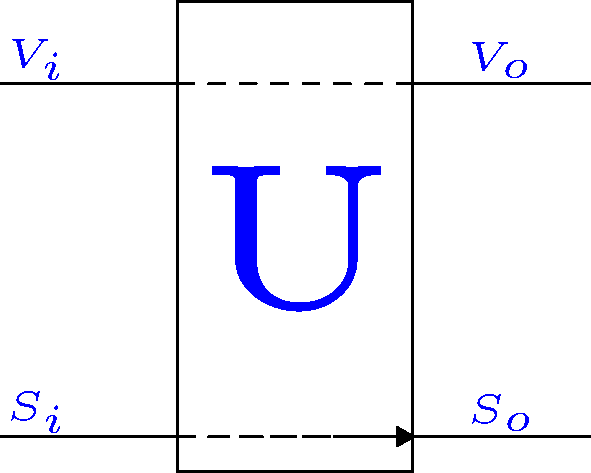
\includegraphics[width=\textwidth]{AbstractSetVerifyUnset}
    \caption{Abstract Unset Set-Verify}
    \vspace{15pt}
    \end{subfigure}
    \hfill
    \begin{subfigure}[b]{0.3\textwidth}
    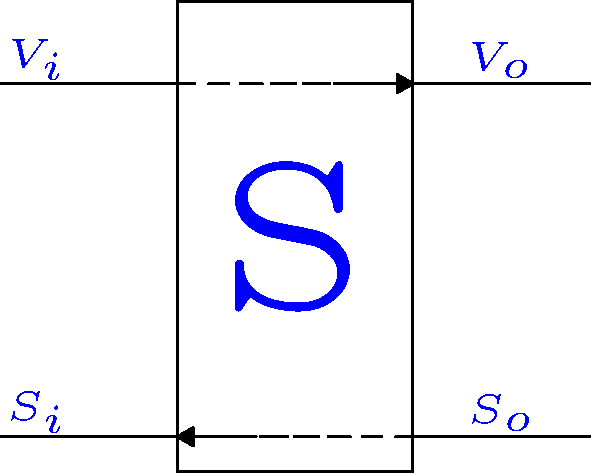
\includegraphics[width=\textwidth]{AbstractSetVerifySet}
    \caption{Abstract Set Set-Verify}
    \vspace{15pt}
    \end{subfigure}
    \hfill
    \begin{subfigure}[b]{0.3\textwidth}
    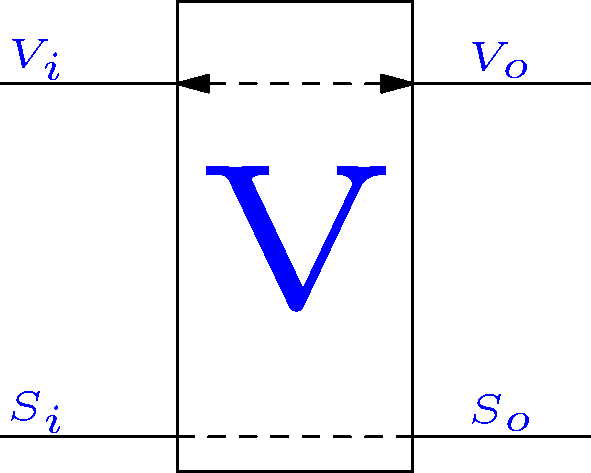
\includegraphics[width=\textwidth]{AbstractSetVerifyVerified}
    \caption{Abstract Verified Set-Verify}
    \vspace{15pt}
  \end{subfigure}  
   \vspace{10pt}
  \begin{subfigure}[b]{0.3\textwidth}
    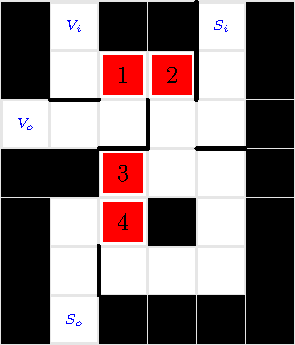
\includegraphics[width=\textwidth]{SetVerifyUnset}
    \caption{Set-Verify, unset state}
    \label{SetVerifyUnset}
  \end{subfigure}
  \hfill
  \begin{subfigure}[b]{0.3\textwidth}
    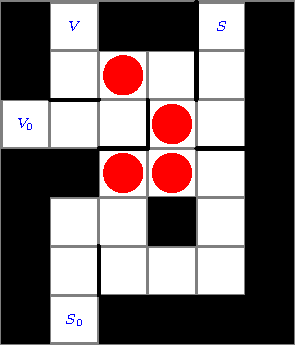
\includegraphics[width=\textwidth]{SetVerifySet}
    \caption{Set-Verify, set state}
    \label{SetVerifySet}
  \end{subfigure}
  \hfill
  \begin{subfigure}[b]{0.3\textwidth}
    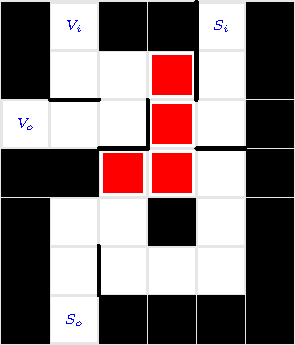
\includegraphics[width=\textwidth]{SetVerifyVerified}
    \caption{Set-Verify, verified state}
    \label{SetVerifyVerified}
  \end{subfigure}
  \caption{Diagrams of three of the states of Set-Verify gadgets along with their construction in a push-pull block puzzle. Red blocks are moveable, black blocks are fixed, thick black lines are thin walls.}
  \label{setVerifyDiagrams}
\end{figure}


\begin{table}
\begin{minipage}{.3\textwidth}
{\setlength\tabcolsep{4pt}
\begin{tabular}{>{$} l <{$} >{$} l <{$} >{$} l <{$} >{$} l <{$}}
   U: & & & \\
   &(U, s_i)& \rightarrow& (S, S_o) \\
\end{tabular}}
\end{minipage}
\begin{minipage}{.3\textwidth}
{\setlength\tabcolsep{4pt}
\begin{tabular}{>{$} l <{$} >{$} l <{$} >{$} l <{$} >{$} l <{$}}
  S: & & & \\
   &(S, s_o)& \rightarrow& (U, S_i) \\
   &(S, v_i)& \rightarrow& (V, v_o) \\
\end{tabular}}
\end{minipage}  
\begin{minipage}{.3\textwidth}
{\setlength\tabcolsep{4pt}
\begin{tabular}{>{$} l <{$} >{$} l <{$} >{$} l <{$} >{$} l <{$}}
   V: & & & \\
   &(V, v_i)& \rightarrow& (V, v_o) \\ 
   &(V, v_o)& \rightarrow& (V, v_i) \\ 
   &(V, v_o)& \rightarrow& (S, v_i) \\ 
\end{tabular}}
\end{minipage}
\caption{State transitions of a Set-Verify gadget as seen in Figure~\ref{setVerifyDiagrams}}
\label{SetVerifyStateTransition}
\end{table}

\subsubsection{Variable and Clause Gadgets}
\label{sec:2DPushPull3SAT}
% Separate variable + clause gadget constructions, keep those here, move stuff about 3SAT specifically to the summary near the end.

We will be making use of the Set-Verify gadget to produce the literals in our 3SAT formula. One significant difficulty with this model is the complete reversibility of all actions. Thus we need to take care to ensure that going backward at any point does not allow the robot to cheat in solving our 3SAT instance. The directional properties of the Set-Verify allow us to create sections where we know if the robot exits, it must have either reset everything to the initial configuration or have correctly proceeded through that gadget.

Our literals will be represented by Set-Verify gadgets, described in Section~\ref{sec:SetVerifyGadgets}. They are considered true when the $V_i$ to $V_o$ traversal is possible, and false otherwise. Thus we can set literals to true by allowing the robot to run through the $S_i$ to $S_o$ passage of the gadget. This allows a simple clause gadget, shown in Figure~\ref{fig:NPClauseGadget}, consisting of splitting the path into three hallways, each with the corresponding verify side of our literal. We can then pass through if any of the literals are set to true, and cannot pass otherwise. Notice that the Unset and Set states do not have a backward transition. Thus the only way to go back through the clause is through the verified literal, after which the clause has been reset to the state it was in before the robot went through it.

The variables will be encoded by a series of passages which split to allow either the true or negated literals to be set, shown in Figure~\ref{fig:NPVariableGadget}. Once the robot has gone through at least one gadget in one hallway, there are only two possibilities remaining: either the robot can continue down the hall setting more literals to true, or the robot can go back through the gadget it has just exited, returning it to its unset state. Thus, before entering or after exiting a hallway all of the literals in that hallway will be in the same state. Additionally, unset gadgets do not allow a transition from $S_o$ to $S_i$, which means at any point while setting variables, if the robot decides to go back it can only return through a hallway which has been switched to the set state. Going back through these returns them to the unset state, putting that variable gadget back in its initial configuration before the robot interacted with it.



\begin{figure}[!ht]
\begin{minipage}{.36\textwidth}
    \includegraphics[width=\textwidth]{NPClauseGadget}
    \caption{Clause gadget, $C_k$, with variables $x_a=1$, $x_b=0$, $x_c=0$.}
    \label{fig:NPClauseGadget}
\end{minipage}
\hspace{5mm}
\begin{minipage}{.57\textwidth}
  \centering
    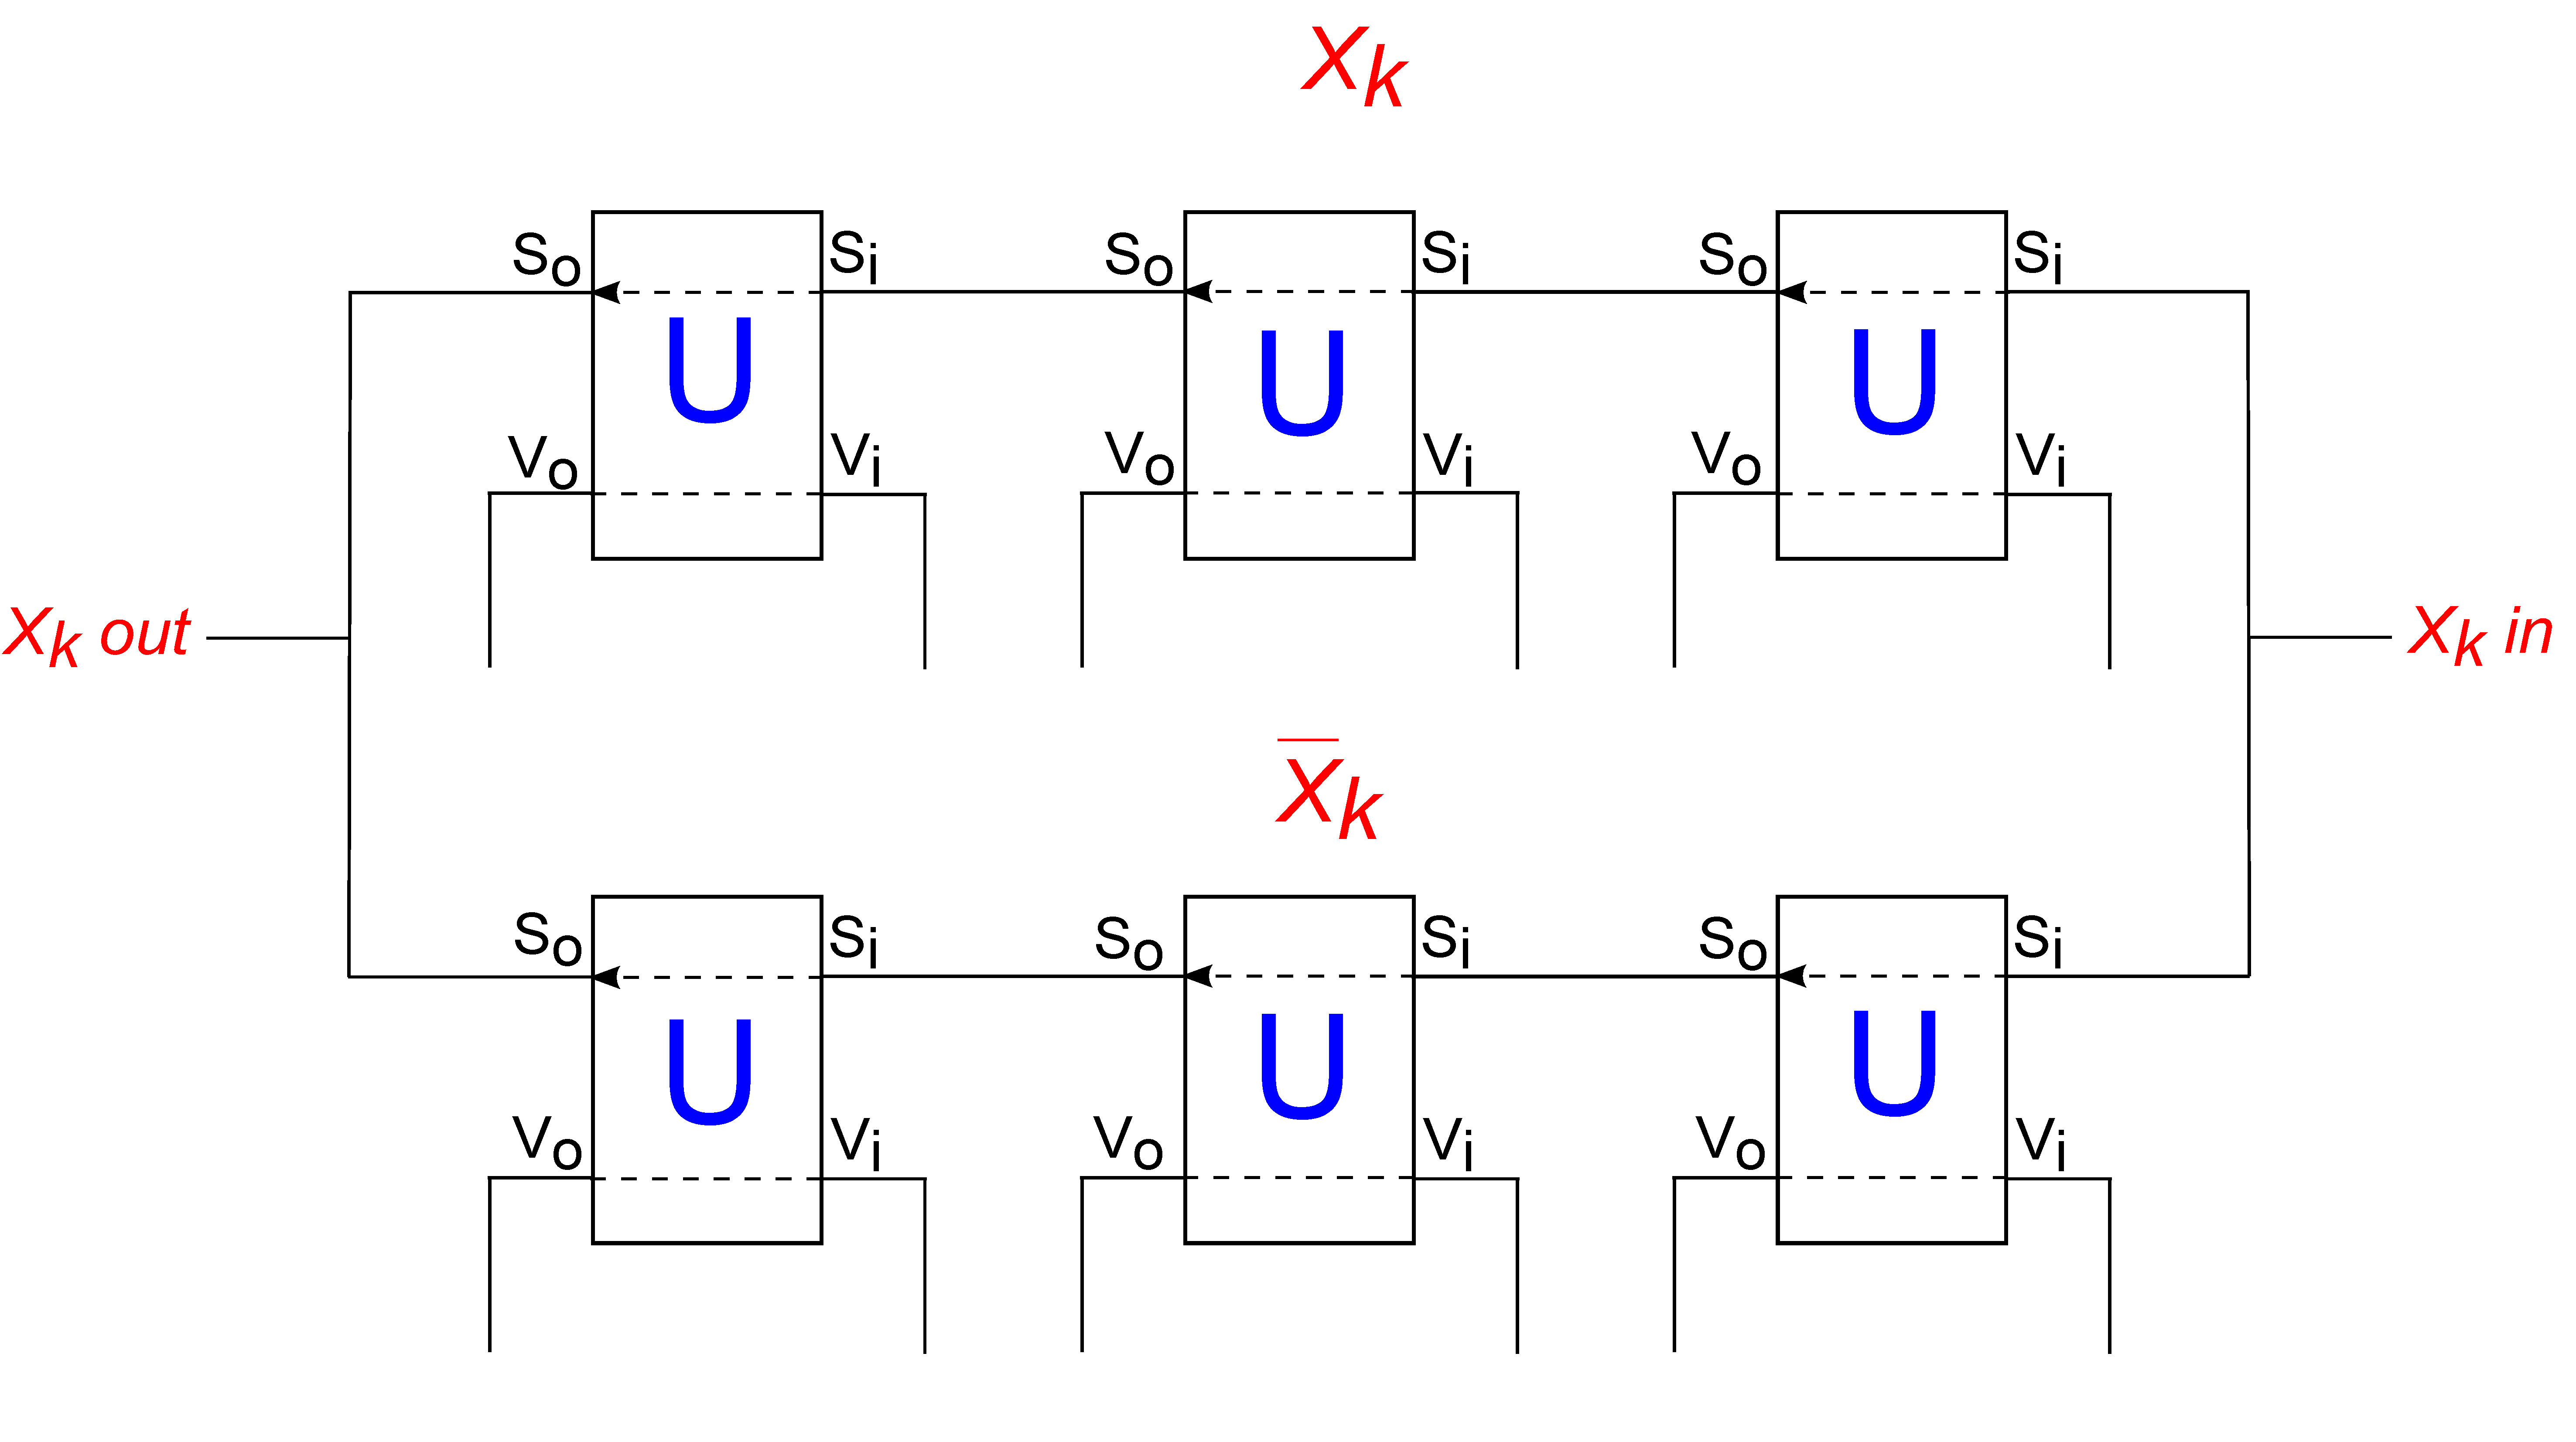
\includegraphics[width=.8\textwidth]{NPVariableGadget}
    \caption{A variable gadget representing $X_k$ occurring in six clauses, three of those times negated. The value of the variable has been set to true.}
    \label{fig:NPVariableGadget}
\end{minipage}
\end{figure}

%\xxx{consider reviving one-way gadget (actually a 1-toggle)}
%\section{Reversible One-Way Gadget}
%When in the initial configuration $A$ the gadget only permits a traversal from $S_o$ to $S_i$ leaving the gadget in configuration $B$. Configuration $B$ only permits traversals in the opposite direction, from $S_i$ to $S_o$. Note, when the robot leave this gadget, the only possible configurations are $A$ and $B$. These gadgets or similar structures will be used several times within more complicated structures.
%
%\begin{figure}[!ht]
%  \centering
%    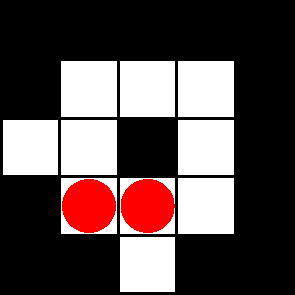
\includegraphics[width=0.8\textwidth]{one_way.pdf}
%    \caption{Reversible one-way gadget.}
%    \label{ldeScreenshotsMap}
%\end{figure}

\subsubsection{Crossover Gadgets}
\label{sec:NPCrossover}
In this section we build up the needed two use crossover gadget from a series of weaker types of crossover gadgets. One may wonder why we need crossover gadgets when Planar 3SAT is NP-complete. This only guarantees that connecting the verticies to their clauses by edges results in a planar graph, it does not ensure that we can navigate our robot between all of these gadgets in a planar manner or that our gadgets themselves are planar. The most obvious issue can be seen in the clause gadget (Figure~\ref{fig:NPClauseGadget}) where one of the Set Verify gadgets must lie between the other two hallways, but must also be accessible by its associated variable gadget.

\paragraph{Directed Destructive Crossover} This gadget, depicted in Figure~\ref{fig:DestructiveCrossover}, allows either a traversal from $a$ to $a'$ or $b$ to $b'$. Once a traversal has occurred, that path may be traversed in reverse, but the other is impassable unless the original traversal is undone.

First, observe that transitions are initially only possible via the $a$ and $b$ entrances, since the transitions possible through a Set-Verify in the Set state can be entered through $V_i$ and $S_o$, not $S_i$. Assume without loss of generality that the gadget is entered at $a$. This changes the state of the left Set-Verify to Verified. At this point, only the right $S_o$ and left $V_o$ transitions are passable. Taking the $V_o$ transition either reverts all changes to the original state, or leaves the left crossover in the Verified state, which allows strictly less future transition than the original state. Therefore, we will disregard that option. Taking the $S_o$ transition changes the right Set-Verify to Unset, and completes the crossover. At this point, the only possible transition is to undo the transition just made, from $a'$ back to $a$, restoring the original state. The gadget could be entered via $a$, but the robot would only be able to leave via $a$, possibly changing the state to Set. Both options result in the robot exiting out its original entrance, and allow the same or less future transtions, so we may disregard those options. Thus, the only transition possibilities are as stated above.

\begin{figure}[!ht]
  \centering
  \begin{subfigure}[b]{0.47\textwidth}
    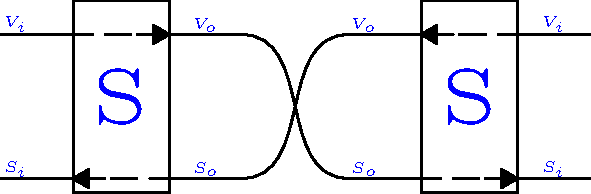
\includegraphics[width=\textwidth]{OneWayDestructiveCrossover}
    \caption{The directed destructive crossover constructed from two connected Set-Verify gadgets initialized in the set position.}
    \label{fig:DestructiveCrossover}
  \end{subfigure}
  \hfill
  \begin{subfigure}[b]{0.47\textwidth}
    \includegraphics[width=\textwidth]{InOrderCrossover}
    \caption{The in-order directed crossover constructed from two connected Set-Verify gadgets initialized in the verified and unset positions.}
    \label{fig:InOrderCrossover}
  \end{subfigure}
  \caption{Two types of crossover gadgets}
\end{figure}

%\begin{figure}[!ht]
%  \centering
%  \begin{subfigure}[b]{0.48\textwidth}
%    \includegraphics[width=\textwidth]{one_use_crossover}
%    \caption{The one use directed crossover is constructed from a directed destructive crossover and two in-order directed crossovers.}
%    \label{OneUseCrossover}
%  \end{subfigure}
%  \hfill
%  \begin{subfigure}[b]{0.43\textwidth}
%    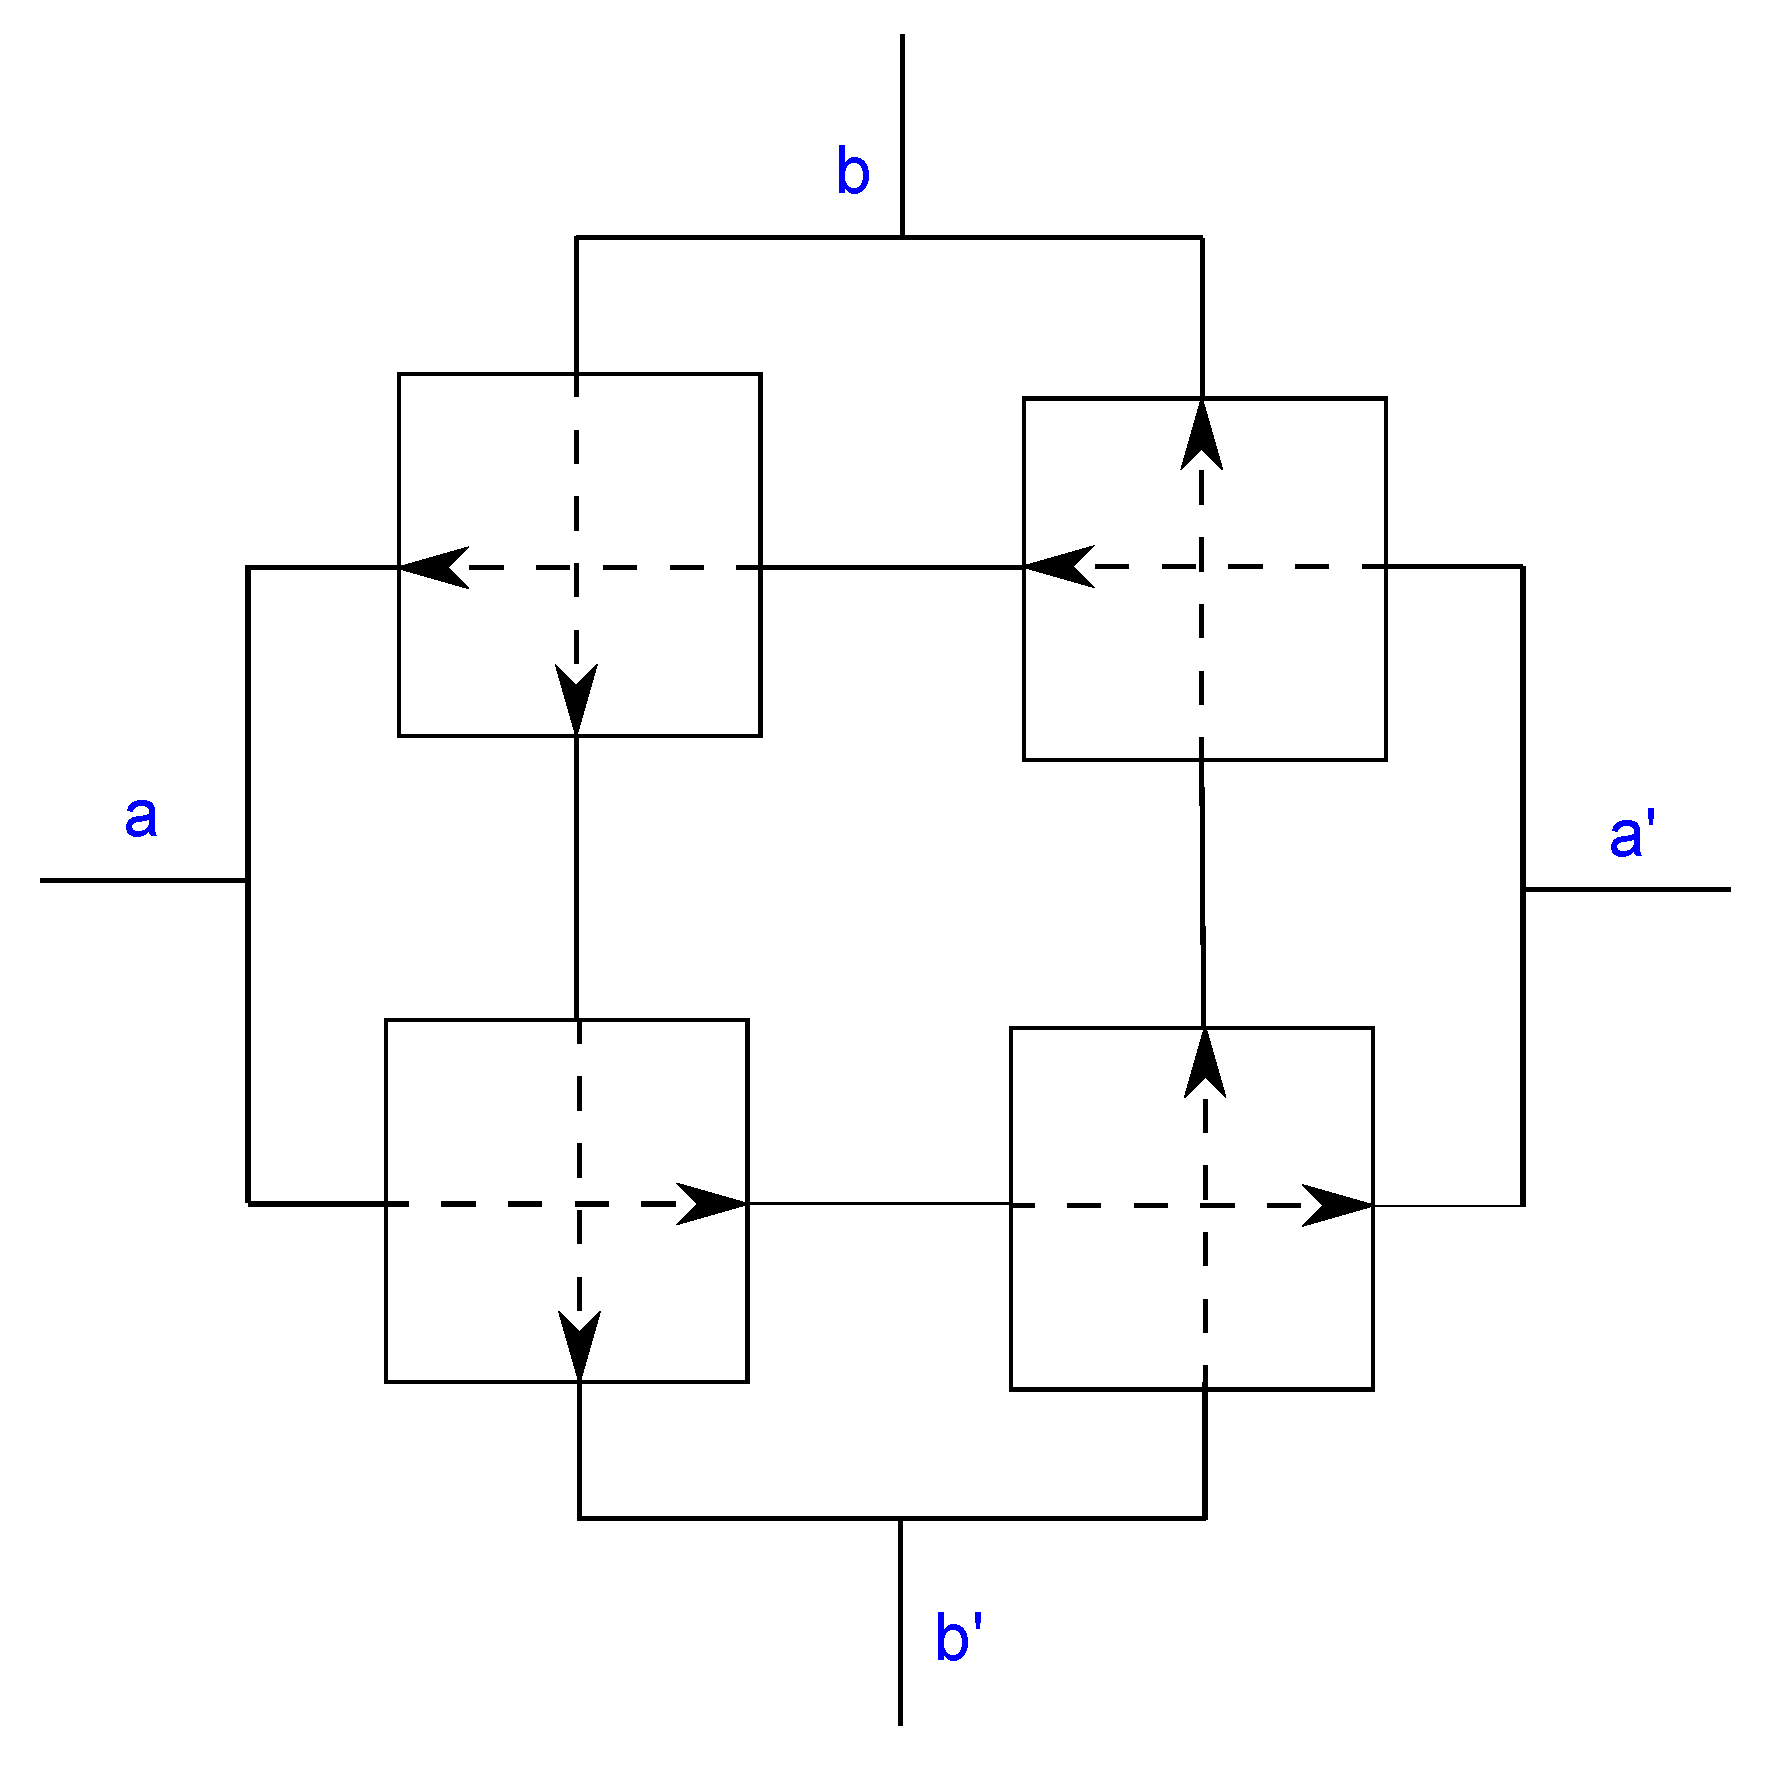
\includegraphics[width=\textwidth]{full_one_use_crossover}
%    \caption{A full one use crossover constructed from four directed one use crossovers.}
%    \label{full_one_use_crossover}
%  \end{subfigure}
%  \caption{Composite crossover gadgets}
%\end{figure}



\paragraph{In-order Directed Crossover} This gadget, depicted in Figure~\ref{fig:InOrderCrossover} allows a traversal from $a$ to $a'$, followed by a traversal from $b$ to $b'$. These traversals may also be reversed.

Initially, no entrance is passable except for $a$, since $V_o$ is passable only in the Verified state, and $S_o$ is
passable only in the Set state. Once the left $V_o \rightarrow V_i$ transition is made, the robot has 2 options.
It can either change the left Set-Verify gadget's state to Set, or leave it as Verified. In either case, the $S_i$
entrance on that toggle is impassable, since a $S_i$ entrance may only be traversed in the Unset state. The
only transition possible on the right crossover is $S_i \rightarrow S_o$, changing the state from Unset to Set.
This completes the first crossing.

Now, there are at most 2 transitions possible: from $a'$ back to $a$, undoing the whole process, or entering at $b$. Note that entering at $b$ is only possible if the left Set-Verify is in the Set state, so let us assume that state change occurred. In that case, the left $S_o \rightarrow S_i$ transition may be performed, changing the left Set-Verify's state to Unset. At that point, the only possible transitions are back to $b$, or through the right Set-Verify's
$V_i \rightarrow V_o$ transition, completing the second crossover.

\begin{wrapfigure}{hr}{0.45\textwidth}
\vspace{-5mm}
  \centering
    \includegraphics[width=.5\textwidth]{one_use_crossover}
    \caption{The two use directed crossover is constructed from a directed destructive crossover and two in-order directed crossovers.}
    \label{fig:OneUseCrossover}
    \vspace{-7mm}
\end{wrapfigure}

If the left Set-Verify was left in the Verify state, strictly less future transitions are possible compared to the case where it was changed into the set state, so we may disregard that possibility.


\paragraph{Two Use Directed Crossover} 
The Two Use Directed Crossover, depicted in Figure~\ref{fig:OneUseCrossover}, is the gadget needed for our proof. It allows a traversal from $a$ to $a'$ followed by a traversal from $b$ to $b'$, or from $b$ to $b'$ and then $a$ to $a'$. These transitions may also be reversed.

It is constructed out of an In-order Directed Crossover gadget and a Destructive Directed Crossover, as shown in Figure~\ref{fig:OneUseCrossover}. The $a$ to $a'$ traversal is initially passable, and goes through both gadgets,
blocking the destructive crossover but leaving the in-order crossover open for the $b$ to $b'$ traversal. If the $a$ to $a'$ traversal does not occur, the $b$ to $b'$ traversal is possible via the destructive crossover.


\begin{wrapfigure}{hr}{0.45\textwidth}
\vspace{-5mm}
  \centering
%  \begin{figure}[t]
%    \centering
    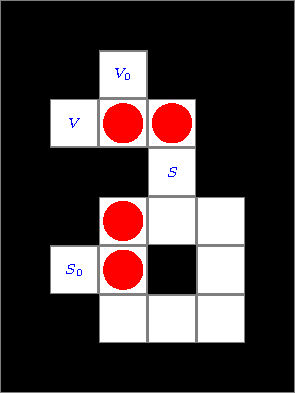
\includegraphics[width=.4\textwidth]{SetVerify3D}
    \caption{A Set-Verify gadget in 3D where the entrances and exits extend upward, notated by the diagonal arrows. This gadget is in the unset state.}
    \label{fig:3DSetVerify}
    \vspace{-12mm}
\end{wrapfigure}


Because of the behavior of the constituent crossovers which make up this gadget, no transition from $a$ to $b$ $a$ to $b'$, etc. is possible. The crossover permits reversal of each of the transitions described, but the crossings can only be reversed in queue order (last in, first out).
%
%\paragraph{Two Use Crossover} 
%Four Directed Crossovers can be combined, as shown below, to create a crossover that can be traversed in any direction \cite{Push100}. This is not necessary for our proof but is shown for general interest. Unfortunately, the inability to go through this gadget multiple times in the same direction without first going back through means it likely isn't sufficient for PSPACE-completeness. 


\begin{theorem}
\label{thm:2DNPhard}
Push-$k$ Pull-$l$ in 2D with thin walls is NP-hard.
\end{theorem}
\begin{proof}
    We will reduce from 3SAT. Given a 3SAT instance with variables $(x_1, x_2, \ldots x_n)$ and clauses $(x_a, x_b, \overline x_c), \ldots$, we will construct an equivalent PushPull instance as follows: 

    First, we will set up the clause gadgets. Each clause gadget will look exactly like Figure~\ref{fig:NPClauseGadget}, with all of the Set-Verify gadgets initially in the unset state. There will be one clause gadget for each clause in the 3SAT formula. The clauses will be linked together in series, $C_k$ $out$ to $C_{k+1}$ in. At the final clause gadget's out exit, we will place the goal square.

    Next, we will set up the variable gadgets. For each variable $x_k$, there will be a variable gadget $X-k$, consisting of a positive literal pathway, connecting to every clause where the variable is used positively, and a negative literal pathway, connecting to every clause where the variable is negated, as shown in Figure~\ref{fig:NPVariableGadget}. These variable gadgets will be linked together in series, $X_k$ $out$ to $X_{k+1}$ $in$. The final variable gadget's $out$ exit will be linked to the first clause gadget's $in$. Just in front of the first variable gadget's $in$ entrance will be the start square.

    The connections between these gadgets will consist of empty hallways, except where such hallways would cross. The hallways inside the clause and variable gadgets will also need to cross, and we will handle them similarly. We need crossovers for this reduction, rather than reducing to a PlanarSAT variant, because we need crossovers just to make the clause gadgets work, as seen here.
    
    At all crossings, we will place a Two Use Directed Crossover, from Figure~\ref{fig:OneUseCrossover}. The orientation of the gadget will be chosen according to a specified ordering, where the later pathway will never be used before the earlier pathway, and no pathway will every be traversed twice in the same direction. The ordering is each variable gadget's hallways, in increasing order of the variable gadgets, followed by each clause gadget's hallways, in increasing order of clause gadgets. Within the variable gadgets, the ordering will be from in to out along the positive and negative lines, with the positive lines arbitrarily placed before the negative lines. The clause gadget hallways won't cross each other.

    With this, the construction is complete. To see that it is solvable if and only if the corresponding SAT problem is satisfiable, first let us consider the case where the SAT problem is satisfiable.

    If the SAT problem is satisfiable, then there is an assignment of variables such that each clause is satisfied, e.g. has at least one true literal. Therefore, the PushPull construction is solvable. It can be solved by traversing each variable gadget via the side corresponding to the satisfying assignment, then traversing each clause, which is passable because it is satisfied. The crossovers do not impede traversal, since the path taken goes through each crossover at most once of each of its pathways, and strictly in the forward direction of the ordering which determined the orientation of the crossovers. Thus, the entire PushPull problem can be solved, as desired.

    Next, let us consider the case where the SAT problem is not satisfiable. Consider a partial traversal of the PushPull problem, from the start cell through the variable gadgets. As described in Section~\ref{sec:2DPushPull3SAT}, regardless of any reverse transitions through a variable gadget or interactions with its clause gadget, if the robot is beyond a given variable gadget, exactly one of the variable lines must be set, and the other must be unset. Likewise, the interactions with the crossover gadgets do not allow any transitions other than within the variable gadgets, regardless of reversals. Moreover, interactions with the clause gadgets only change the state of Set-Verify gadgets corresponding to literals between the Set and Verified states. If a Set-Verify is Unset, its state cannot be altered via its verify line ($V_i - V_o$).

    Thus, regardless of the robot's prior movements, the only literals that will be Set or Verified are at most those corresponding to a single assignment for each variable. No two literals corresponding to opposite assignments of the same variable will every be in the Set or Verified states at the same time. 

    Since the SAT problem is assumed to be unsatisfiable, no assignment of variables will satisfy every clause. Thus, as the robot exits the variable gadgets and enters the clause gadgets, for any prior sequence of moves, there must be some clause gadget which has all of its literals in the Unset state, corresponding to the unsatisfied clause for this setting of variables. Since all clauses must be traversed to reach the goal cell, and a clause cannot be traversed if all of its literals are Unset, the robot cannot reach the goal cell. Thus, the PushPull problem is unsolvable.

    We have demonstrated that the PushPull problem is solvable if and only if the corresponding 3SAT instance is satisfiable. The reduction mentioned above is polynomial time reduction, as long as the hallways are constructed reasonably. Thus, Push-$k$ Pull-$l$ in 2D with thin walls is NP-hard.


\end{proof}


\subsection{3D Push-Pull is NP-hard}
\label{3DNPhard}
In this section we prove that 3D Push-$k$ Pull-$l$ with fixed blocks is NP-hard, for all positive $k$ and $l$. All of the hard work was done in the previous section. Here we will simply show how we can use the additional dimension to tweak the previous gadgets to build them without thin walls. We reduce from 3SAT, constructing our variables from chains of 3D Set-Verify gadgets, and our clauses from the verify side of the corresponding 3D Set-Verify gadget.

\begin{theorem}
3D Push-$k$ Pull-$l$ with fixed blocks is NP-hard, for all positive $k$ and $l$.
\end{theorem}
\begin{proof}
We follow the proof of Theorem~\ref{thm:2DNPhard} using a modified Set-Verify gadget, shown in Figure~\ref{fig:3DSetVerify}.  It can be easily checked that this has the same properties as the Set-Verify given in Section~\ref{sec:SetVerifyGadgets}. We do note that the cyclic ordering of the entrances in the 3D Set-Verify is different from that of the 2D Set-Verify, however this is not important as we no longer need to construct crossovers. With a functional Set-Verify gadget, the remaining constructions of variables and clauses proceeded as in Section \ref{sec:2DPushPull3SAT}. No crossover gadgets are needed since we are working in 3D. Finally, we note that all blocks are in hallways of length at most 3, thus the gadgets still function as described for any positive push and pull values.

%As before, in the unset state the only possible traversal is $S_i$ to $S_0$. This traversal allows the top right bock to be pulled down, moving the gadget into the set state. From here the $V$ to $V_0$ traversal is possible, as well as going back through the $S_0$ to $S$ pathway. However, the $S$ to $S_0$ traversal is not possible.

%Variables are composed of hallways of 3D Set-Verify gadgets connected $S_0$ to $S$, one for each clause in which the variable appears, as in Figure~\ref{fig:NPVariableGadget}. Clauses are composed of three 3D Set-Verify gadgets connected in parallel as in Figure~\ref{fig:NPClauseGadget}. The details of these constructions follow those in Section~\ref{sec:2DPushPull3SAT} This completes the reduction from 3SAT. In addition, we note that all blocks are in hallways of length at most 3, thus the gadgets still function as described for any positive push and pull values.
\end{proof}
